\documentclass[UTF8]{beamer}
\usepackage{ctex} % 支持中文
\usepackage{amsmath}
\usepackage{amssymb} % For symbols like \mathbb{E}, \lim, \sum
\usepackage{amsthm} % For proof environments if needed (though not strictly used here)

% --- Theme and Appearance ---
\usetheme{Madrid} % A popular, clean theme
% \usetheme{AnnArbor} % Another good option
% \usetheme{Singapore} % Yet another option
\usecolortheme{default} % Or try others like 'whale', 'orchid'

% Remove navigation symbols ( uncomment if you want them)
\setbeamertemplate{navigation symbols}{}

% --- Custom Colors for Beamer Blocks ---
% Using standard Beamer blocks like 'block' and 'alertblock'
% Let's redefine their colors to be distinct but match the theme style somewhat.
\setbeamercolor{block title}{bg=blue!20!white, fg=black} % Default block title color
\setbeamercolor{block body}{bg=blue!5!white, fg=black}   % Default block body color

\setbeamercolor{example title}{bg=green!20!white, fg=black} % Custom for 'example' blocks
\setbeamercolor{example body}{bg=green!5!white, fg=black}

\setbeamercolor{alertblock title}{bg=red!20!white, fg=black}   % Alert block title color
\setbeamercolor{alertblock body}{bg=red!5!white, fg=black}     % Alert block body color


% --- Define math operators for better typography ---
\DeclareMathOperator{\E}{\operatorname{E}}
\DeclareMathOperator{\Var}{\operatorname{Var}}
\DeclareMathOperator{\Prob}{\operatorname{P}}

\title{第七讲 大数定律}
\author{龚鹤扬}
\institute{中国科学技术大学统计学博士 \\ 上海芯梯科技有限公司} % Using \institute is standard for affiliation, split lines with \\
\date{\today}

\begin{document}

\begin{frame}
    \titlepage
\end{frame}

\begin{frame}{目录}
    \tableofcontents
\end{frame}

\section{引言}
\begin{frame}[shrink=10]{引言:大数定律的重要性与局限}
    \framesubtitle{并非对所有随机变量都成立的普适规律}
    \begin{itemize}
        \item 本讲讨论概率论中一组重要的极限定理——\alert{大数定律 (Law of Large Numbers, LLN)}。
        \item 核心思想:在大量重复试验中,事件发生的\alert{频率}近似于其\alert{概率},样本均值收敛于总体\alert{期望}。
        \item 大数定律是连接\alert{理论概率}与\alert{统计推断}的桥梁,为许多统计方法的合理性提供了理论基础。
        \item \alert{重要提示}:大数定律的结论依赖于随机变量满足特定的\alert{条件}(例如,期望存在、方差有限等)。
        \item 并非所有随机变量序列都满足这些条件。本讲将以一个著名的反例——\alert{柯西分布 (Cauchy distribution)}为例,深入探讨条件的必要性。
    \end{itemize}
\end{frame}

\section{切比雪夫不等式}
% Shrink may be needed if content is too much
\begin{frame}[shrink=5]{7.1 切比雪夫不等式 (Chebyshev's Inequality)}
    \framesubtitle{一个重要的概率上界}
    \begin{itemize}
        \item 切比雪夫不等式给出了随机变量偏离其期望值的概率的一个\alert{上界}。
        \item 这个界不依赖于随机变量的具体分布形式,只需要其\alert{期望}和\alert{方差}存在且有限。
    \end{itemize}
    \pause
    \begin{block}{定理 7.1 (切比雪夫不等式)}
        设随机变量 X 具有期望 $\E(X) = \mu$ 和方差 $\Var(X) = \sigma^2$ (其中 $0 < \sigma^2 < +\infty$)。
        则对于任意正数 $\epsilon > 0$,有:
        \[ \Prob(|X - \mu| \geq \epsilon) \leq \frac{\sigma^2}{\epsilon^2} \]
        或者等价地:
        \[ \Prob(|X - \mu| < \epsilon) \geq 1 - \frac{\sigma^2}{\epsilon^2} \]
    \end{block}
    \pause
    \textbf{意义与特点:}
    \begin{itemize}
        \item \alert{普适性}:对任何分布都成立(只要期望、方差存在)。
        \item \alert{实用性}:在分布未知时,可以提供一个粗略的估计。
        \item \alert{局限性}:通常这个界比较宽松,即估计可能不够精确。
    \end{itemize}
\end{frame}

\section{弱大数定律 (WLLN)}
% Shrink may be needed if content is too much
\begin{frame}[shrink=5]{7.2 弱大数定律 (Weak Law of Large Numbers, WLLN)}
    \framesubtitle{样本均值的依概率收敛}
    弱大数定律 (WLLN) 表明,在特定条件下,当试验次数 $n$ 足够大时,样本均值 \alert{依概率收敛} 于总体期望。
    \vspace{0.3cm}

    \begin{block}{定理 7.2 (切比雪夫弱大数定律)}
        设 $X_1, X_2, \dots, X_n, \dots$ 是一列\alert{相互独立}、具有相同期望 $\E(X_i) = \mu$ 和相同\alert{有限方差} $\Var(X_i) = \sigma^2 < +\infty$ 的随机变量序列。
        令样本均值为 $\bar{X}_n = \frac{1}{n} \sum_{i=1}^{n} X_i$。
        则对于任意 $\epsilon > 0$,有:
        \[ \lim_{n \to \infty} \Prob(|\bar{X}_n - \mu| \geq \epsilon) = 0 \]
        或者等价地:
        \[ \lim_{n \to \infty} \Prob(|\bar{X}_n - \mu| < \epsilon) = 1 \]
        这表示样本均值 $\bar{X}_n$ \alert{依概率收敛}于 $\mu$,记作 $\bar{X}_n \xrightarrow{P} \mu$。
    \end{block}
    \vspace{0.3cm}
    \footnotesize
    \textit{注:此定理依赖于方差存在且有限,并通过切比雪夫不等式证明。}
\end{frame}

\begin{frame}{伯努利弱大数定律}
    \framesubtitle{频率的稳定性}
    \begin{block}{定理 7.3 (伯努利弱大数定律)}
        设 $n_A$ 是 $n$ 次独立重复伯努利试验中事件 A 发生的次数,$p$ 是事件 A 在每次试验中发生的概率。
        令 $f_n = \frac{n_A}{n}$ 为事件 A 发生的频率。
        则对于任意 $\epsilon > 0$,有:
        \[ \lim_{n \to \infty} \Prob\left(\left| f_n - p \right| \geq \epsilon\right) = 0 \]
        伯努利大数定律揭示了"\alert{频率稳定性}"的本质:当试验次数 $n$ 很大时,事件的频率 $f_n$ 会以很高的概率接近其真实的概率 $p$。
    \end{block}
    \vspace{0.3cm}
    \footnotesize
    \textit{注:伯努利大数定律是切比雪夫弱大数定律的一个重要特例,为用频率估计概率提供了理论依据。}
\end{frame}

% 新增幻灯片:引入柯西分布
\begin{frame}[shrink=10]{期望存在的重要性:引入柯西分布}
    \framesubtitle{一个大数定律不成立的著名反例}
    \begin{itemize}
        \item 我们看到,切比雪夫弱大数定律要求方差存在且有限。许多其他版本的大数定律则要求更弱但依然关键的条件:\alert{期望的存在性}。
        \item 那么,是否存在期望不存在的随机变量? \alert{是的,柯西分布就是一个典型例子。}
    \end{itemize}
    \pause
    \begin{columns}[T] % Top-align columns
        \begin{column}{0.55\textwidth}
            \begin{block}{柯西分布 (Cauchy Distribution)}
                一个更普适的柯西分布的概率密度函数 (PDF) 定义为:
                \[ f(x; x_0, \gamma) = \frac{1}{\pi\gamma \left[1 + \left(\frac{x-x_0}{\gamma}\right)^2\right]} \]
                其中 $x_0 \in (-\infty, +\infty)$ 是位置参数 (决定峰值位置,也是中位数和众数),
                $\gamma > 0$ 是尺度参数 (决定分布的宽度,半峰全宽)。
                
                当 $x_0=0, \gamma=1$ 时,即为标准柯西分布: $f(x) = \frac{1}{\pi (1+x^2)}$。
                \textbf{特点:}
                \begin{itemize}
                    \item 形状类似钟形(对称于 $x_0$),但尾部比正态分布"厚得多"(重尾)。
                    \item \alert{期望 $\E(X)$ 不存在}:对于任意 $x_0, \gamma$,其期望积分 $\int_{-\infty}^{\infty} x f(x; x_0, \gamma) dx$ 仍然是发散的(更准确地说,绝对期望发散)。
                    \item \alert{方差 $\Var(X)$ 也不存在} (因为它依赖于期望)。
                \end{itemize}
            \end{block}
        \end{column}
        \begin{column}{0.4\textwidth}
            \begin{figure}
                \centering
                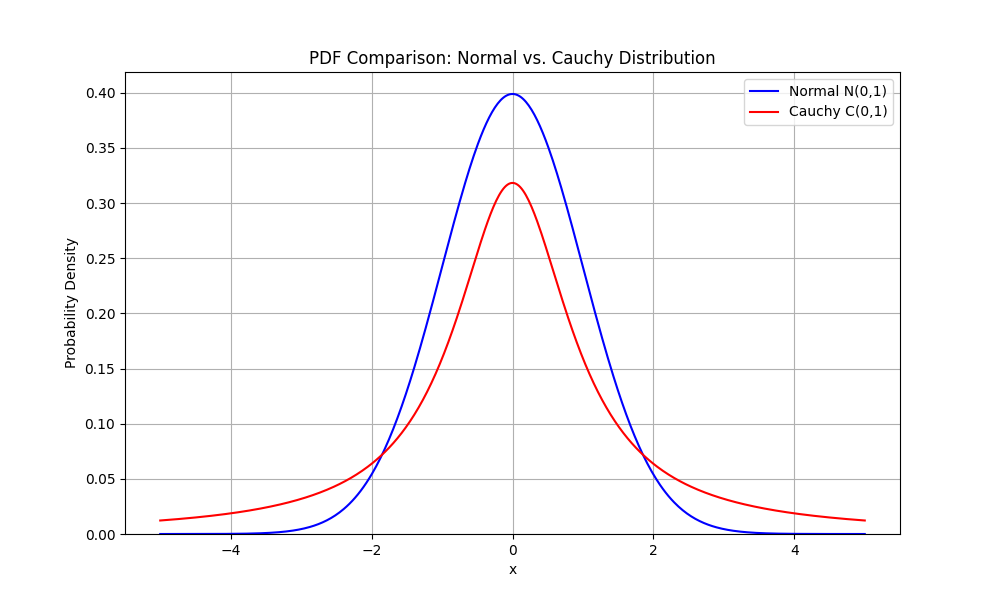
\includegraphics[width=\linewidth]{pdf_normal_cauchy_comparison.png} % Width relative to column
                \caption*{PDFs: N(0,1) vs C(0,1)} % Shortened, unnumbered caption
            \end{figure}
        \end{column}
    \end{columns}
    \pause % Moved after the columns
    \textbf{这意味着什么?}
    \begin{itemize}
        \item 柯西分布不满足绝大多数大数定律版本所要求的"期望存在"或"方差有限"的条件。
        \item 我们将看到,对于 i.i.d. 柯西分布的随机变量序列,它们的样本均值\alert{不会}收敛到任何常数。
    \end{itemize}
\end{frame}

% Inserted from gemini_2_5pro.tex
\begin{frame}[shrink=10]{可视化:正态 vs. 柯西样本均值路径}
    \framesubtitle{样本均值随样本量 $n$ 变化的轨迹}
    \begin{columns}[T] % T for top alignment
        \begin{column}{0.5\textwidth}
            \centering
            \textbf{正态分布 $N(0,1)$}\\($\E(X)=0$, $\Var(X)=1$)
            \begin{figure}
                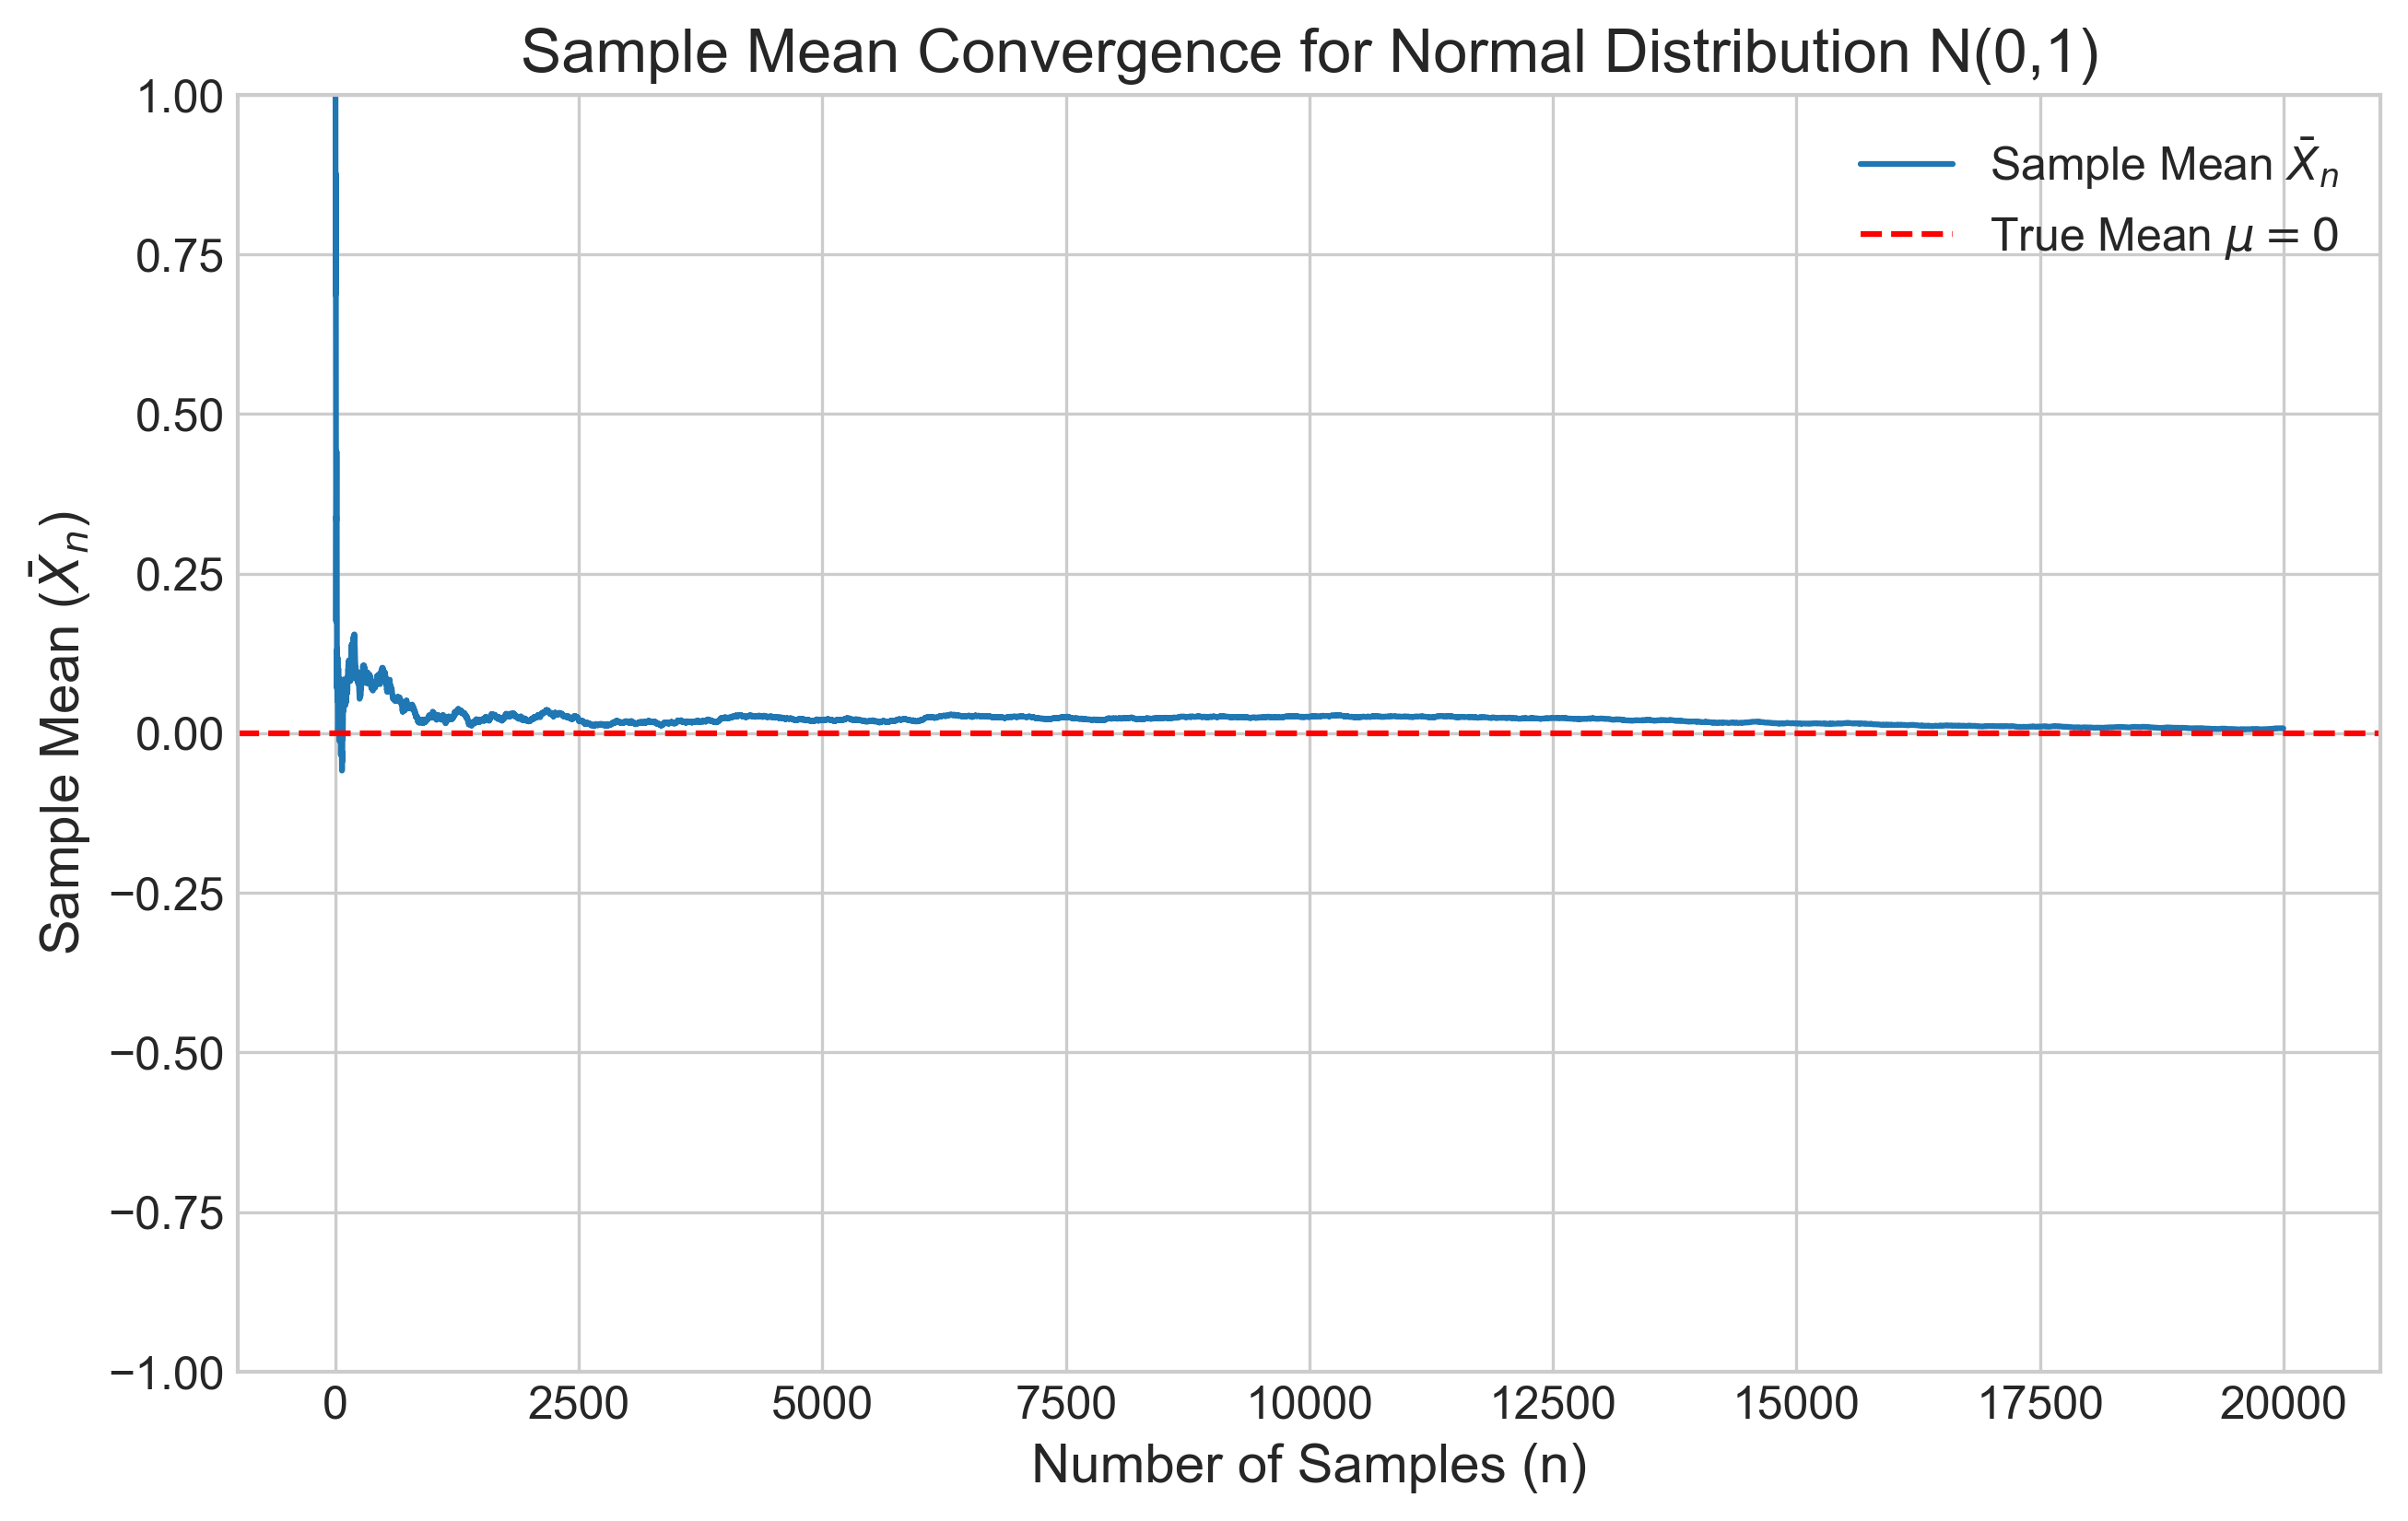
\includegraphics[width=\linewidth]{normal_mean_convergence.png}
                \caption{$\bar{X}_n$ 快速稳定收敛到 $\mu=0$}
            \end{figure}
        \end{column}
        \begin{column}{0.5\textwidth}
            \centering
            \textbf{柯西分布 $C(0,1)$}\\($\E(X)$ 不存在)
            \begin{figure}
                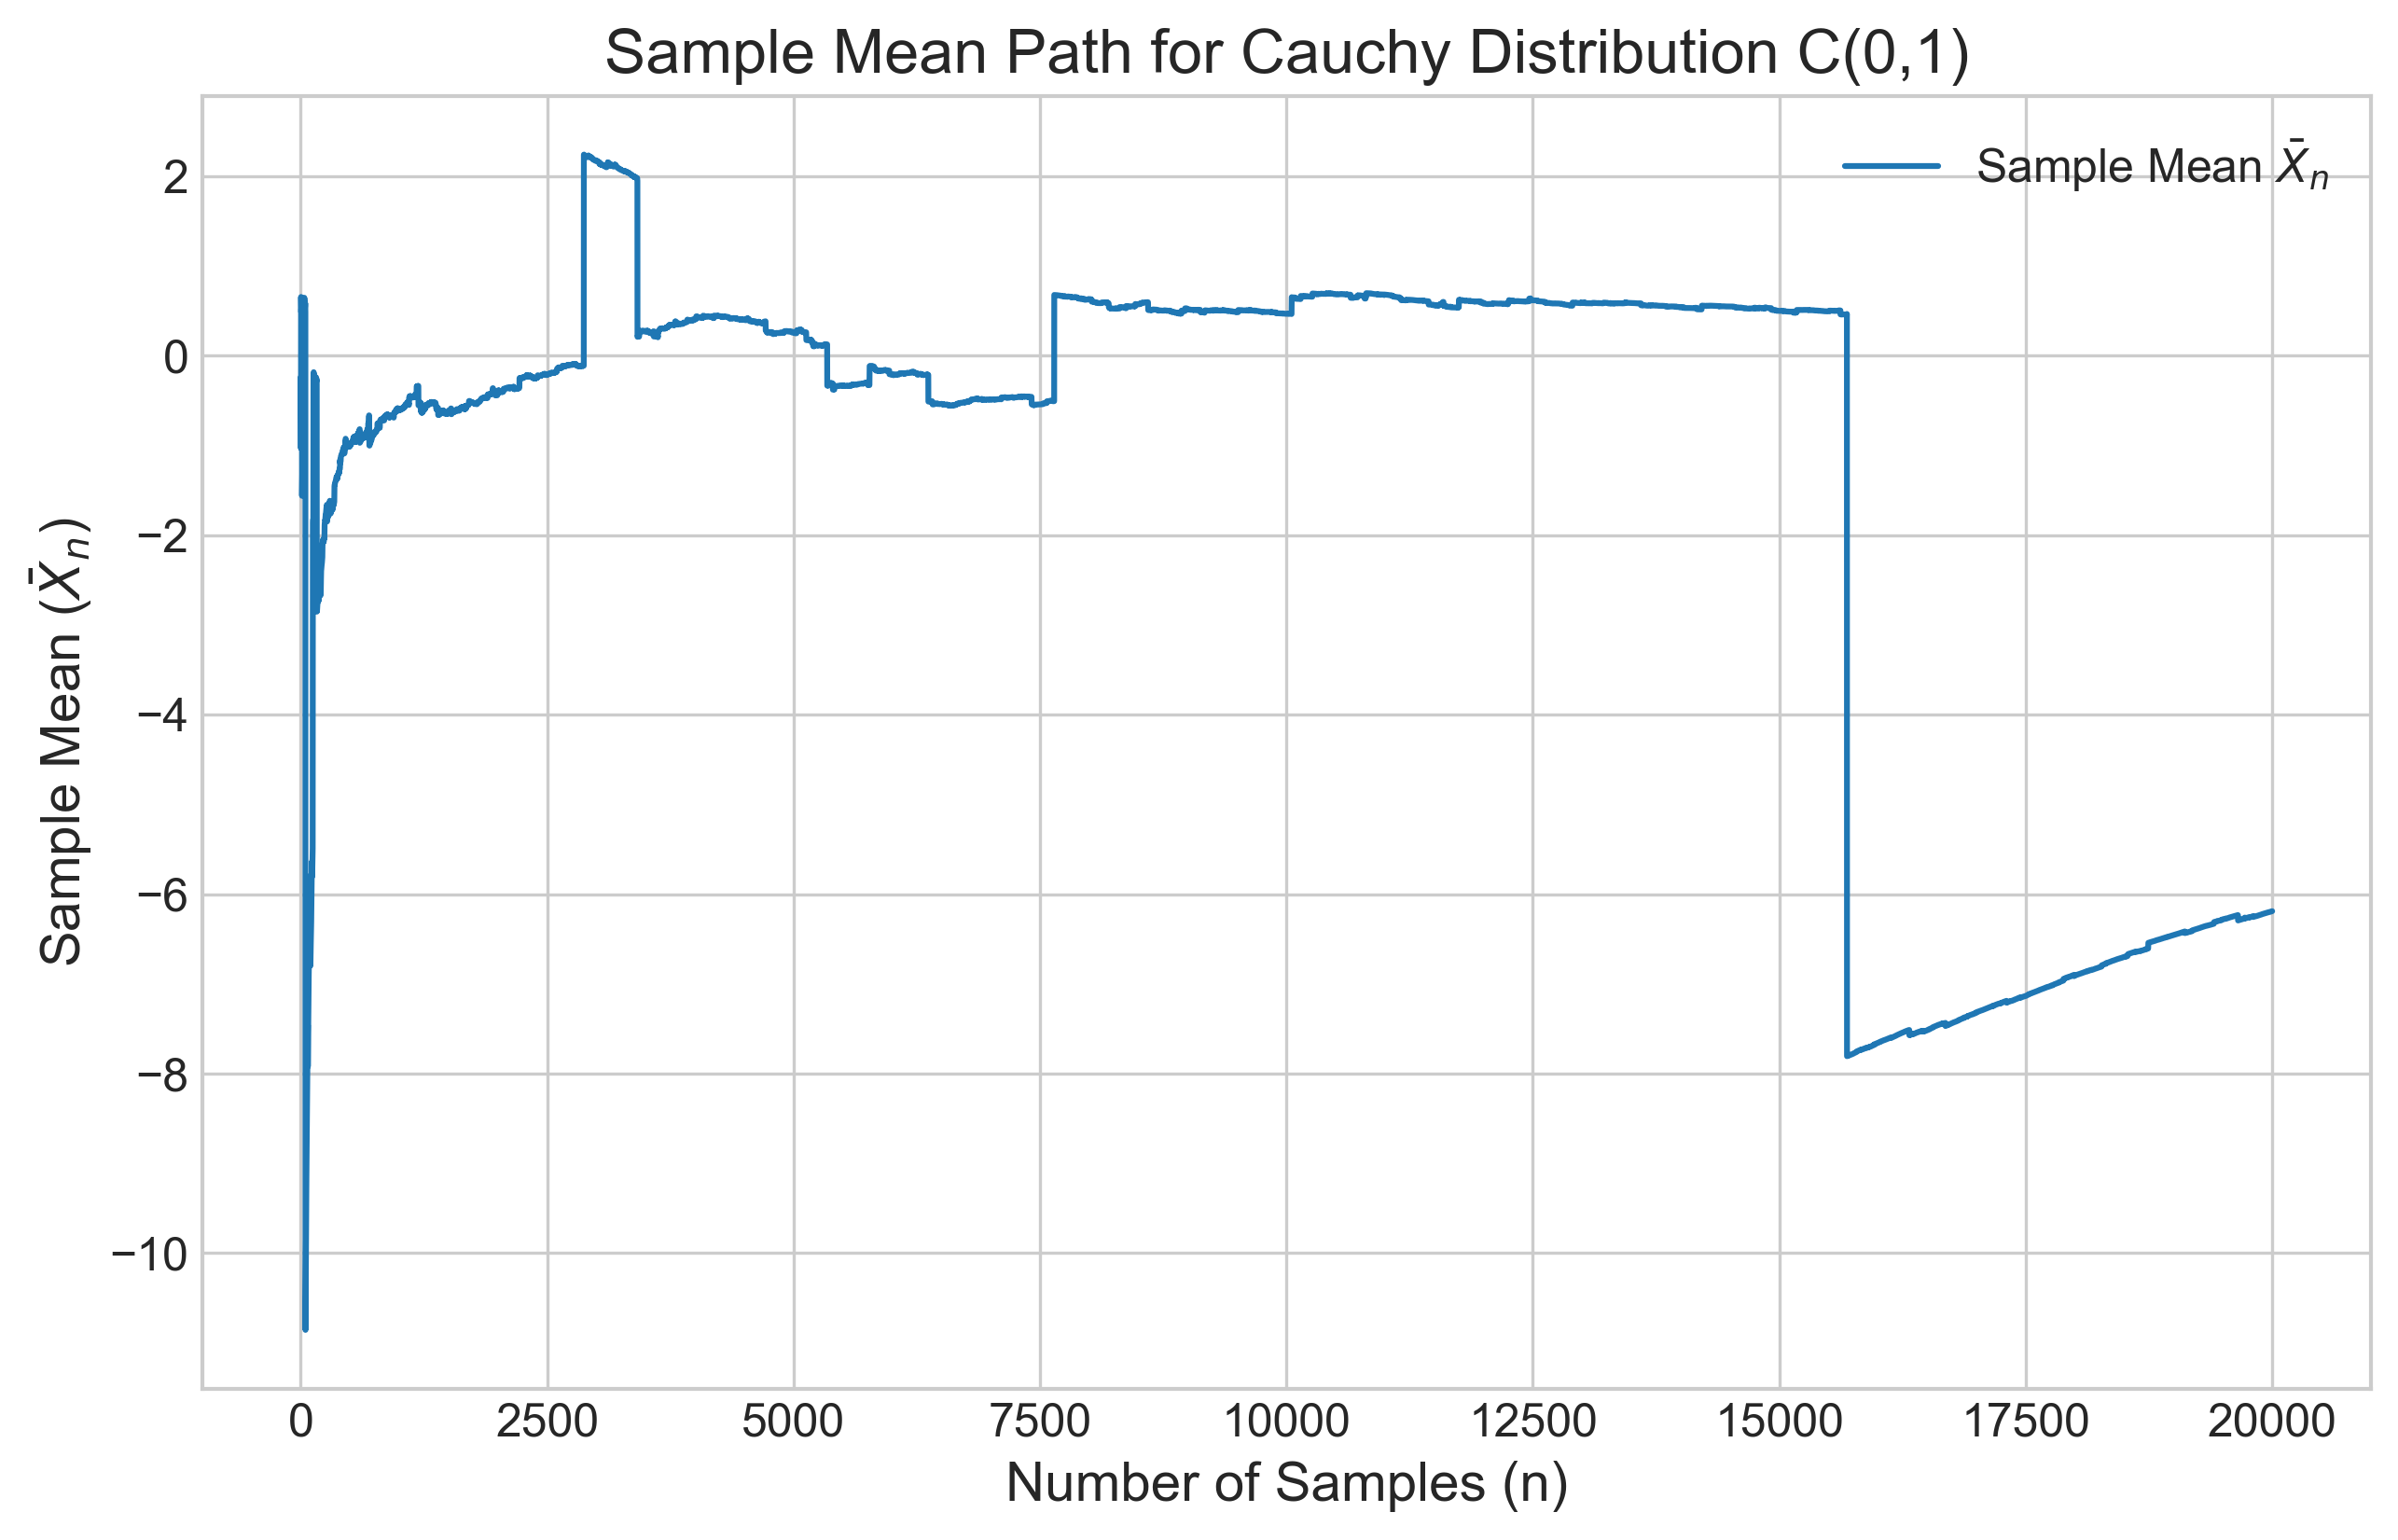
\includegraphics[width=\linewidth]{cauchy_mean_no_convergence.png}
                \caption{$\bar{X}_n$ 持续剧烈波动, \alert{不收敛}}
            \end{figure}
        \end{column}
    \end{columns}
    \vspace{0.2cm}
    \textbf{观察与结论:}
    \begin{itemize}
        \item 正态分布的样本均值行为良好,符合大数定律预期。
        \item 柯西分布的极端值持续"污染"样本均值,使其无法稳定。
    \end{itemize}
\end{frame}
% End of inserted content

% 修改辛钦弱大数定律幻灯片
\begin{frame}[shrink=10]{7.2 弱大数定律 (续):辛钦弱大数定律 (Khinchin's WLLN)}
    \framesubtitle{期望存在即可保证依概率收敛 (i.i.d.情况)}
    辛钦弱大数定律对随机变量序列的方差要求更低,仅要求期望存在且序列是独立同分布的。
    \vspace{0.3cm}
    \begin{block}{定理 7.4 (辛钦弱大数定律)} % Number changed to 7.4
        设 $X_1, X_2, \dots, X_n, \dots$ 是一列\alert{独立同分布 (i.i.d.)} 的随机变量序列,且其共同的期望 $\E(X_i) = \mu$ \alert{存在} (即 $|\mu| < \infty$)。
        令样本均值为 $\bar{X}_n = \frac{1}{n} \sum_{i=1}^{n} X_i$。
        则对于任意 $\epsilon > 0$,有:
        \[ \lim_{n \to \infty} \Prob(|\bar{X}_n - \mu| \geq \epsilon) = 0 \]
        即 $\bar{X}_n \xrightarrow{P} \mu$。
    \end{block}
    \vspace{0.3cm}
    \textbf{回顾柯西分布:}
    \begin{itemize}
        \item 柯西分布是 i.i.d. 序列,但其期望\alert{不存在}。
        \item 因此,i.i.d.柯西随机变量序列\alert{不满足}辛钦弱大数定律的条件。
        \item 其样本均值 $\bar{X}_n$ \alert{不会}依概率收敛到任何常数 $\mu$。这与定律的结论相反。
    \end{itemize}
\end{frame}


\section{强大数定律 (SLLN)}
% 修改强大数定律幻灯片
\begin{frame}[shrink=10]{7.3 强大数定律 (Strong Law of Large Numbers, SLLN)}
    \framesubtitle{样本均值的几乎必然收敛 (更强的收敛)}
    强大数定律 (SLLN) 比弱大数定律具有更强的收敛性,它表明样本均值 \alert{几乎必然收敛} (或称以概率1收敛) 于总体期望,同样要求期望存在。
    \vspace{0.3cm}

    \begin{block}{定理 7.5 (柯尔莫哥洛夫强大数定律)} % Number changed to 7.5
        设 $X_1, X_2, \dots, X_n, \dots$ 是一列\alert{独立同分布 (i.i.d.)} 的随机变量序列,且其共同的期望 $\E(X_i) = \mu$ \alert{存在} (即 $|\mu| < \infty$) 。
        令样本均值为 $\bar{X}_n = \frac{1}{n} \sum_{i=1}^{n} X_i$。则:
        \[ \Prob\left( \lim_{n \to \infty} \bar{X}_n = \mu \right) = 1 \]
        这表示样本均值 $\bar{X}_n$ \alert{几乎处处收敛} (Almost Surely Converge) 于 $\mu$,记作 $\bar{X}_n \xrightarrow{a.s.} \mu$。
    \end{block}
    \vspace{0.3cm}
    \textbf{再次回顾柯西分布:}
    \begin{itemize}
        \item 柯西分布的期望\alert{不存在}。
        \item 因此,i.i.d.柯西随机变量序列\alert{不满足}柯尔莫哥洛夫强大数定律的条件。
        \item 其样本均值 $\bar{X}_n$ \alert{不会}几乎必然收敛到任何常数。
    \end{itemize}
    \footnotesize
    \textit{注:柯尔莫哥洛夫强大数定律的条件与辛钦弱大数定律相同 (i.i.d.且期望存在),但结论更强。}
\end{frame}

% 修改WLLN 与 SLLN 的区别与联系幻灯片:加入正态 vs 柯西对比
\begin{frame}[shrink=5]{WLLN 与 SLLN 的区别与联系 (1):核心概念与正态分布}
    \framesubtitle{依概率收敛 vs. 几乎必然收敛}
    \textbf{核心区别}:
    \begin{itemize}
        \item \textbf{弱大数定律 (WLLN) - \alert{依概率收敛} ($\xrightarrow{P}$)}: $\lim_{n \to \infty} \Prob(|\bar{X}_n - \mu| \geq \epsilon) = 0$. 描述的是\alert{概率}趋于1。
        \item \textbf{强大数定律 (SLLN) - \alert{几乎必然收敛} ($\xrightarrow{a.s.}$)}: $\Prob(\lim_{n \to \infty} \bar{X}_n = \mu) = 1$. 描述的是\alert{样本路径}的极限行为。
    \end{itemize}
    \pause
    \textbf{条件与对比:}
    \begin{itemize}
        \item SLLN 比 WLLN \alert{更强} ($\xrightarrow{a.s.} \implies \xrightarrow{P}$)。
        \item 两者最广泛应用的 i.i.d. 版本都要求 \alert{期望存在} ($|\mu| < \infty$)。
        \item \textbf{对于正态分布 (例如 $N(\mu, \sigma^2)$):}
            \begin{itemize}
                \item 期望 $\mu$ 存在,方差 $\sigma^2$ 有限。满足大数定律条件。
                \item i.i.d.正态随机变量的样本均值 $\bar{X}_n$ \alert{依概率收敛} 且 \alert{几乎必然收敛} 于其期望 $\mu$。
            \end{itemize}
%        \item \textbf{对于柯西分布:}
%            \begin{itemize}
%                \item 期望\alert{不存在}。不满足大数定律的期望存在条件。
%                \item i.i.d.柯西随机变量的样本均值 $\bar{X}_n$ \alert{不}依概率收敛于任何常数。
%                \item i.i.d.柯西随机变量的样本均值 $\bar{X}_n$ \alert{不}几乎必然收敛于任何常数。
%                \item \alert{惊人事实}:若 $X_1, \dots, X_n$ i.i.d. 服从标准柯西分布,则它们的样本均值 $\bar{X}_n = \frac{1}{n} \sum_{i=1}^n X_i$ \alert{仍服从标准柯西分布}! (与 $n$ 无关)
%            \end{itemize}
    \end{itemize}
\end{frame}

\begin{frame}[shrink=5]{WLLN 与 SLLN 的区别与联系 (2):柯西分布反例}
    \framesubtitle{期望不存在导致大数定律失效}
    \textbf{回顾柯西分布的关键特性:}
     \begin{itemize}
        \item 期望\alert{不存在}。因此不满足大数定律的期望存在条件。
    \end{itemize}
    \pause
    \textbf{对于柯西分布的样本均值:}
    \begin{itemize}
        \item i.i.d.柯西随机变量的样本均值 $\bar{X}_n$ \alert{不}依概率收敛于任何常数。
        \item i.i.d.柯西随机变量的样本均值 $\bar{X}_n$ \alert{不}几乎必然收敛于任何常数。
        \item \alert{惊人事实}:若 $X_1, \dots, X_n$ i.i.d. 服从标准柯西分布,则它们的样本均值 $\bar{X}_n = \frac{1}{n} \sum_{i=1}^n X_i$ \alert{仍服从标准柯西分布}! (与 $n$ 无关)
    \end{itemize}
    \vspace{0.3cm}
    \textit{这与满足大数定律条件的正态分布形成了鲜明对比,突出了期望存在性对于大数定律的重要性。}
\end{frame}

\section{大数定律的应用}
% Shrink may be needed
\begin{frame}[shrink=5]{7.4 大数定律的应用 (Applications of LLN)}
    \framesubtitle{应用的基础:满足定律的条件}
    大数定律是概率论与数理统计之间重要的理论基石,应用广泛:
    \begin{itemize}
        \item \textbf{前提}:这些应用都隐式或显式地假设了相关的随机变量序列满足大数定律的条件 (通常是期望存在)。
        \item \textbf{理论基础与解释现象}:
            \begin{itemize}
                \item \alert{频率的稳定性}:为用频率近似概率提供了理论依据 (伯努利大数定律)。
                \item 解释了在大量重复试验中,随机事件的平均结果会趋于一个稳定的值。
            \end{itemize}
        \item \textbf{统计推断}:
            \begin{itemize}
                \item \alert{参数估计}:样本均值是总体期望的\alert{一致估计量}。这是矩估计法等参数估计方法的基础。\alert{但只有当总体期望存在时才成立!}
                \item \alert{蒙特卡洛方法}:通过大量随机抽样来估计积分、期望等数值解。依赖于"样本均值逼近期望"的性质。
            \end{itemize}
        \item \textbf{风险管理与保险}:预测平均赔付,依赖于平均结果的稳定性。
        \item \textbf{质量控制与抽样检验}:根据样本均值推断总体均值或合格率,依赖于样本均值的收敛性。
        \item \textbf{物理与工程}:测量误差的分析:多次测量的平均值通常比单次测量更接近真实值。
            \begin{itemize}
                \item \textit{如果测量误差服从柯西分布,那么增加测量次数并计算平均值是\alert{没有帮助的},因为平均值不会收敛到真实值,甚至其分布形状都不变!}
            \end{itemize}
    \end{itemize}
    \textbf{大数定律的条件(尤其是期望存在)是其应用有效性的关键。对于像柯西分布这样期望不存在的情况,基于样本均值的大数定律应用会失效。}
\end{frame}

\section{总结与展望}
% Shrink may be needed
\begin{frame}[shrink=5]{总结与展望}
    \begin{block}{本讲小结}
        \begin{itemize}
            \item \textbf{切比雪夫不等式}:提供了概率的通用上界(需方差存在)。
            \item \textbf{大数定律}:样本均值在特定条件下收敛于总体期望。
                \begin{itemize}
                    \item \textbf{弱大数定律 (WLLN)}:依概率收敛 ($\xrightarrow{P}$)。辛钦WLLN要求i.i.d.且期望存在。
                    \item \textbf{强大数定律 (SLLN)}:几乎必然收敛 ($\xrightarrow{a.s.}$)。柯尔莫哥洛夫SLLN要求i.i.d.且期望存在。结论更强。
                \end{itemize}
            \item \alert{\textbf{条件的重要性}}:大数定律的结论依赖于随机变量满足特定条件,最核心的是\alert{期望的存在性}。
            \item \alert{\textbf{反例:柯西分布}}
                \begin{itemize}
                    \item 柯西分布的期望\alert{不存在}。
                    \item 因此,i.i.d.柯西变量的样本均值\alert{不服从}大数定律,不会收敛到任何常数。
                    \item 柯西分布的样本均值\alert{仍服从}柯西分布,突显了期望不存在时的特殊行为。
                \end{itemize}
            \item 大数定律是连接概率论与统计实践的\alert{核心桥梁},理解其条件和局限性对于正确应用至关重要。
        \end{itemize}
    \end{block}
\end{frame}

\begin{frame}
    \begin{alertblock}{展望}
        \begin{itemize}
            \item 大数定律描述了\alert{平均}行为的极限。
            \item 另一类核心极限定理是\alert{中心极限定理 (CLT)},它描述了样本均值(或和)的\alert{分布}趋向于正态分布。它也通常要求期望和方差存在。
            \item 大数定律和中心极限定理共同构成了现代统计推断的理论基石。
        \end{itemize}
    \end{alertblock}
\end{frame}

\begin{frame}
    \centering
    \Huge{\bfseries 谢谢聆听!}
    \vspace{1cm}
    \normalsize
    问题与讨论
\end{frame}

\end{document}